\documentclass[a4paper,oneside,dvipsnames]{article}

\pagenumbering{gobble}

\usepackage{epigraph}
\usepackage[hidelinks]{hyperref}
\usepackage{mathtools}
\usepackage{amsfonts}
\usepackage{graphicx}
\usepackage{xcolor}
\usepackage{tabu}
\usepackage{enumitem}
\usepackage{textcomp}
\usepackage{upquote}
\usepackage{caption}

\usepackage{float}

\usepackage[margin=2.5cm,textwidth=15cm]{geometry}
\usepackage[many]{tcolorbox}

\usepackage{minted}
\usepackage[T1]{fontenc}
\usepackage{lmodern}

\usepackage{tikz}
\usetikzlibrary{trees}

% http://tex.stackexchange.com/questions/112559/box-around-minted-environment/112573#112573
% =========================================================================================
\usepackage{etoolbox}
\BeforeBeginEnvironment{minted}{\begin{tcolorbox}}%
\AfterEndEnvironment{minted}{\end{tcolorbox}}%
\usepackage{lineno}
\def\gobble#1{}
\renewcommand\DeleteFile[1]{}
\usepackage{xparse}
\ExplSyntaxOn
\box_new:N \l_fvrb_box
\tl_new:N \l_fvrb_tl
\RenewDocumentCommand \FancyVerbFormatLine { m }
 {
   \hbox_set:Nn \l_fvrb_box { #1 }
    \dim_compare:nNnTF { \box_wd:N \l_fvrb_box }>{ \linewidth }
      {%box to big 
       \tl_set:Nn \l_fvrb_tl { #1 }
       \fvrb_use_tl:N \l_fvrb_tl
      } 
      {%box fits
       \box_use:N \l_fvrb_box
      }
 }
\cs_new:Npn \fvrb_use_tl:N  #1
 {
  \group_begin:
   \null\hfill\vbox_set:Nn \l_fvrb_box
     {\hsize=\linewidth
      \renewcommand\thelinenumber
           {
             \ifnum\value{linenumber}=1\relax\else
                  $\rightarrow$
             \fi
           }
      \begin{internallinenumbers}
        \advance\hsize by -2em
        \hspace*{-2em}\tl_use:N #1
      \end{internallinenumbers}
     }
   \box_use:N \l_fvrb_box
  \group_end:
}
\ExplSyntaxOff
% =========================================================================================


\usepackage[utf8x]{inputenc}
\pagenumbering{arabic}

\begin{document}

\begin{titlepage}

\title{Deep Reinforcement Learning}
\author{
\\\\SoftServe Data Science Group\\\\
\definecolor{light-gray}{gray}{0.3}
{\small {Ihor Kostiuk, Roman Grubnyk, Iurii Milovanov, Ievgenii Baliuk, Pavlo Kramarenko, Chris Poulin}}\\
{\small {DSG\makeatletter @\makeatother softserveinc.com}}\\
{\small {v.02}}
\\\\
}
\date{}
\clearpage\maketitle
\thispagestyle{empty}

\end{titlepage}

\tikzstyle{every node}=[draw=black,thick,anchor=west]
\tikzstyle{selected}=[draw=red,fill=red!30]
\tikzstyle{optional}=[dashed,fill=gray!50]
\tableofcontents
\newpage

\epigraph{What is our life? A game!}{The Queen of Spades\\ by Pyotr Ilyich Tchaikovsky}


\section[Introduction]{Introduction}

Although games are usually undertaken for enjoyment, they are also used as an educational tool or as a tool for simulating complex life situations for training in critical thinking and decision making. Now there are a great variety of games ranging from competitive sports, to board and video games, or even mind training focused games. Each game has its individual type, form, and structure.
\\

While for much of their history, other humans were the logical opponent for games. But in early 1950s, when the Era of the Personal Computer came, this restriction was removed. The computer has become number-one opponent. Since then there was an enormous amount of competitions which tried to estimate a human brain’s abilities in playing games in comparison to the state of the art computer algorithms. 
\footnote{\url{http://en.wikipedia.org/wiki/Watson\_(computer)\#Jeopardy.21}}
\footnote{\url{http://en.wikipedia.org/wiki/Deep\_Blue\_versus\_Garry\_Kasparov}}
Although there was a great progress in developing such ‘opponent agents’ during the last years, the main goal of our project lies in the artificial intelligence of the `human player simulating' game playing agent.
\\

The DeepMind
\footnote{\url{http://deepmind.com/}} 
team had recently proposed to use Convolution Neural Networks to extract features from raw data (without any hand written features). This new `unsupervised learning' approach provides a huge flexibility and algorithm abilities increase in order to work on different data and solve different problems, with noteworthy performance. \\

With credit to the prior projects by Deepmind
\footnote{\url{http://www.cs.toronto.edu/\~vmnih/docs/dqn.pdf}}
% \ and the University of Tartu, Estonia
% \footnote{\url{https://courses.cs.ut.ee/MTAT.03.291/2014\_spring/uploads/Main/Replicating\%20DeepMind.pdf}}
, our Data Science Group has also decided to develop a solution which would be able to achieve at or better performance in playing video games with computer than an expert human player. Our main goal is to completely generalize this idea and make it able to be applied to any video game. This particular use case could become a breakthrough in the study of Artificial Intelligence.


\noindent
\section[Theory]{Theory}
At this time, we are not about to introduce any new mathematical ideas or concepts in our project. Rather we want to put together currently existing state-of-the-art approaches and techniques to achieve a higher goal by combining them. In this chapter we will briefly explain the main underlying concepts of our solution such as Reinforcement Learning and Neural Networks, to let you understand ‘how it actually works’. [Note: There will be a great deal of math and other process descriptions, so feel free to skip this section and jump directly to \hyperref[sec:implementation]{Implementation} (or even \hyperref[sec:gettingStarted]{Getting Started with DRL}) if you're already familiar with these concepts.]


\subsection[Reinforcement Learning]{Reinforcement Learning}
Reinforcement Learning (RL)
\footnote{\url{http://en.wikipedia.org/wiki/Reinforcement\_learning}}
\ is the set of algorithms (or approaches) inspired by behaviorist psychology. The idea behind it is that a computer algorithm (hereafter, agent) interacts with some unknown or semi-known environment (may be stochastic) using predefined and limited set of actions in a way that maximize some cumulative reward. The environment is typically formulated in terms of Markov Decision Process (MDP) \footnote{\url{http://en.wikipedia.org/wiki/Markov\_decision\_process}}. It defines an environment $\varepsilon$ as a two finite sets:
\begin{itemize}
    \item $S = \{s_1,\dots,s_n\}$ -- set of environment internal states;
    \item $A = \{a_1,\dots,a_k\}$ -- set of environment legal actions;
    \item $\delta : S \times A \to S$ -- transition function (usually unknown);
\end{itemize}
An agent interacts with environment $\varepsilon$ in discrete time steps. On each step $t$ in a state $s_t$ it chooses an action $a_t \in A$ which is subsequently sent as a command to the environment. The environment changes agent's state from $s_t$ to $s_{t+1}$. As a result of transition $[s_t, a_t, s_{t+1}]$ (means: from state $s_t$ to state $s_{t+1}$ by taking action $a_t$) agent immediately receives a reward $r_{t+1}$. The reward given by environment often is discounted by some so-called discount-factor $0\leq\gamma\leq1$.
Thus we can define an expected discounted return after game termination by:
\begin{equation} \label{eq:reward}
    R = \sum_{t=0}^{N} \gamma^t r_{t+1}
\end{equation}
here, $N$ is the game termination time.\\\\
The agent makes its decisions on action to be taken in order to maximize an expected reward by following some action-value function which calculates quality of a state-action pair with respect to the past experience:
\begin{equation} \label{eq:quality}
    Q : S \times A \to R
\end{equation}
Based on Bellman equation of optimality, we can define the optimal action-value function  $Q^*(s,a)$ as the maximum expected reward for the state-action pair $(s,a)$ achievable by taking action $a$ in state $s$ and thereafter following an optimal strategy by maximizing the expected value of $r + \gamma Q^*(s', a')$:
\begin{equation} \label{eq:quality}
    Q^*(s,a) = \mathbb{E}_{s'\sim \varepsilon}[r + \gamma \max_{a'} Q^*(s', a')|s,a]
\end{equation}
The problem of optimal strategy determination, based on formulated optimization criterion, is referred to the dynamic programming problems. There are two general approaches:
\begin{itemize}
    \item Iteration by strategy
    \item Iteration by values
\end{itemize}
Both approaches are computer-intensive, especially when power of possible states and action sets is significant enough. It explains inappropriateness of using traditional algorithms, when Markov Decision Process is reduced to hidden Markov model. In this case we can apply some approximate approaches, and one of the most successful solutions is applying Q-learning approximation by using apparatus of artificial neural networks.\\
The agent follows a greedy strategy on action selection $a = \max_{a} Q(s, a)$.  However it can randomize its selection to explore states that have not been visited yet. Thus we define the $\epsilon$-greedy strategy that follows the greedy strategy with probability $1 -− \epsilon$ and selects a random action with probability $\epsilon$.

\subsection[Neural Networks]{Neural Networks}
Artificial Neural Networks (ANNs) are mathematical models inspired by biological neural networks and are limited imitation of human's central nervous system (in particular the brain). In Machine Learning
\footnote{\url{http://en.wikipedia.org/wiki/Machine\_learning}}
they are used as an approach to approximate functions $f : X \to Y$ (usually non-linear) by "learning" it from large amount of input data.

\subsubsection[Architecture]{Architecture}
There is a variety of approaches to build Neural Network topology, but in our project we consider only feedforward approach
\footnote{\url{http://en.wikipedia.org/wiki/Feedforward\_neural\_network}}.
It contains following basic elements:
\begin{itemize}
    \item Nodes (known as neurons) connected together by directed links to form a network;
    \item Connections between neurons associated with weights;
    \item Layers composed of neurons;
\end{itemize}
A connection from neuron $i$ to neuron $j$ propagates the activation $a$ from $i$ to $j$. Each connection also has a numeric weight $w_{i,j}$ associated with it, which determines the strength of the link. Each neuron $j$, in order to calculate its activation value $a_j$, first computes a weighted sum of all of its inputs, and then applies an activation function $g$ to it:
\begin{equation} \label{eq:activation}
    a_j = g(\sum_{i=0}^{n} w_{i,j} a_i)
\end{equation}
The activation function could be:
\begin{itemize}
    \item sigmoid function
    \footnote{\url{http://en.wikipedia.org/wiki/Sigmoid\_function}}.
    \item linear function
    \footnote{\url{http://en.wikipedia.org/wiki/Linear\_function}}.
    \item other advanced techniques (such as SoftMax, MaxOut etc)
\end{itemize}
Neural Networks usually are arranged in multiple layers of nodes in a directed graph, with each layer fully connected to the next one. The first one usually is called as Input layer and the final layer the Output layer. Intermediate layers of nodes between the Input and Output layers called the Hidden layer. The activation values on input layer represent the data input and the output layer activations represent the result value. The hidden layers are responsible for intermediate calculations that fit to the underlying data structure. The number of neurons in each layer depends on the amount of input data and the type (or complexity) of problem being solved.
\begin{figure}[h]
    \centering
    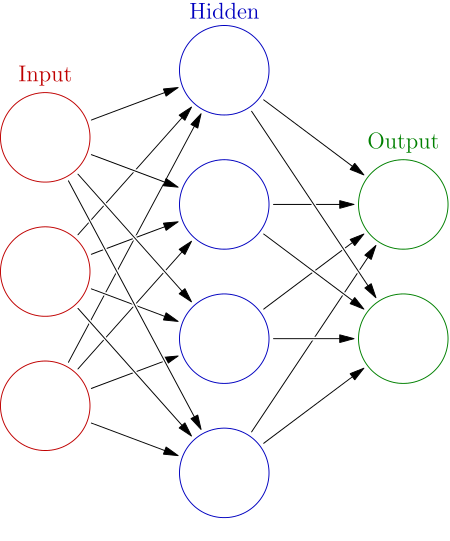
\includegraphics[scale=0.39]{450px-Colored_neural_network.png}
    \caption{Neural network}
    \label{fig:awesome_image}
\end{figure}


\subsubsection[Training]{Training}
In Neural Networks learning occurs in changing connection weights by minimizing the Loss function. This is an example of supervised learning, and is carried out through backpropagation technique
\footnote{\url{http://en.wikipedia.org/wiki/Backpropagation}}
\ in conjunction with an optimization method such as gradient descent.

\subsection[Deep Learning]{Deep Learning}
Deep learning is an area of machine learning which is composed of a set of algorithms and techniques that attempt to define the underlying dependencies in a data and to model its high-level abstractions. The main goal of this approach is to avoid manual description of a data structure (like hand-written features) by automatic learning it from the data. Its name refers to the fact that typically any Neural Network with two or more hidden layers is called deep neural network. Deep Learning techniques usually are applied to the tasks on a data which is not easy to represent as a valuable set of features because of its complexity (such as image or audio signal). Thus its main field of application lies in computer vision and speech recognition.

\subsubsection[Convolutional Neural Networks]{Convolutional Neural Networks}
Convolutional neural network is a deep learning technique which is now widely used in image recognition. Architecturally, it is a type of feed-forward artificial neural network where the individual neurons are tiled in such a way that they respond to overlapping regions in the visual field. \footnote{\url{http://en.wikipedia.org/wiki/Convolutional\_neural\_network\#cite\_note-deeplearning-1}}
\begin{figure}[h]
    \centering
    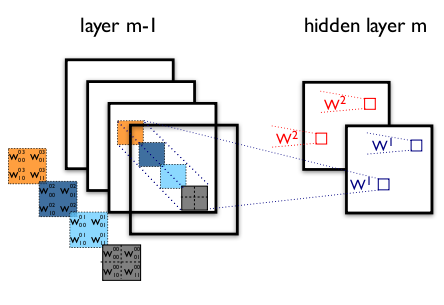
\includegraphics[scale=0.9]{cnn_explained.png}
    \caption{Convolutional neural network}
    \label{fig:cnn_explained}
\end{figure}
\\
Convolutional neural networks consists of a combination of multiple hidden layers of small cells of neurons which look specifically at small frame of the input image. The results of these cells are then tiled so that they overlap to obtain a better representation of the original image; this is repeated for every such layer. Because of this, they are able to tolerate translation of the input image. \footnote{\url{http://citeseerx.ist.psu.edu/viewdoc/summary?doi=10.1.1.125.3812}} These cells act as local filters over the input space and are well-suited to exploit the strong spatially local correlation present in natural images.\\\\
Convolutional neural networks also implement a few important concepts (such as Shared Weights
\footnote{\url{http://deeplearning.net/tutorial/lenet.html\#shared-weights}}
and MaxPooling
\footnote{\url{http://deeplearning.net/tutorial/lenet.html\#maxpooling}}
) that bring a big advantage in a field of Deep Learning and Computer Vision.
\begin{figure}[H] 
    \centering
    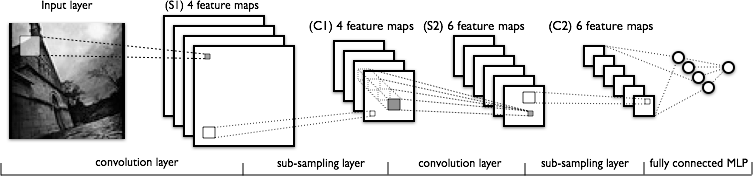
\includegraphics[scale=0.8]{mylenet.png}
    \caption{Full-stack model example}
    \label{fig:mylenet}
\end{figure}

\newpage
\noindent
\section[Implementation]{Implementation}
\label{sec:implementation}

\subsection[Process description]{Process description}
\subsubsection[Explanation]{Explanation}

The Diagram below (Figure \ref{fig:nn_map}) illustrates the flow of ‘train and predict’ functionality of the neural
network. The blocks, marked by blue color and numbering are suggestions for future improvement. Meanwhile, there are also explanatory notes with benefits of each, with links for corresponding papers in chapter \ref{subsec:improvements}.

\begin{figure}[h]
    \centering
    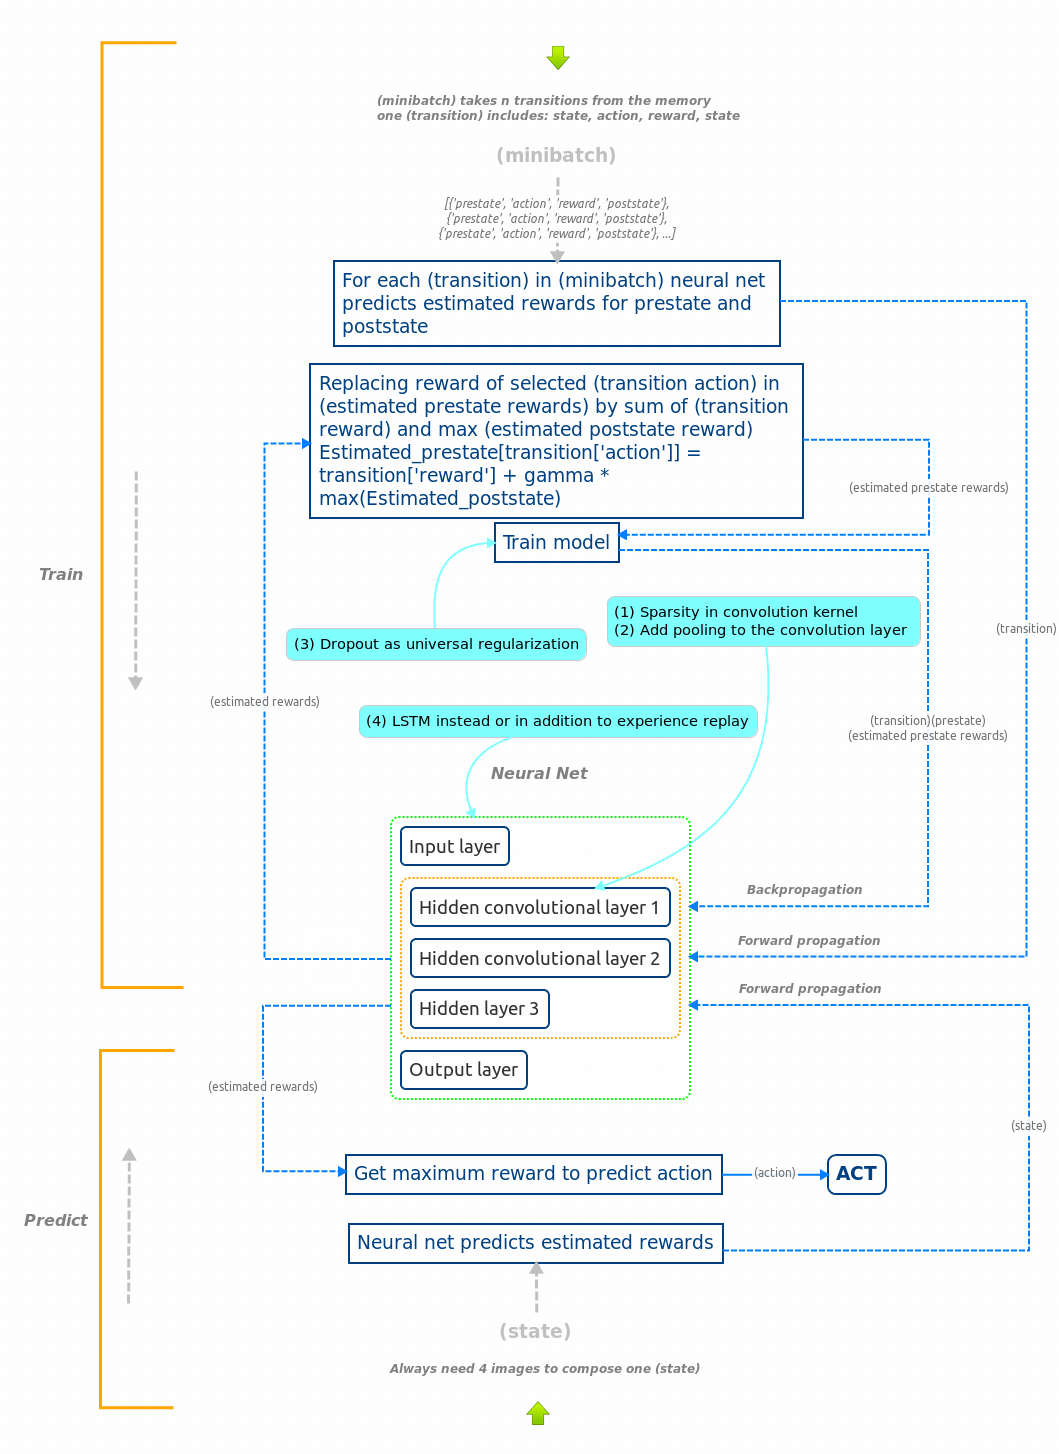
\includegraphics[scale=0.3]{nn_map.png}
    \caption{Learning diagram}
    \label{fig:nn_map}
\end{figure}

\subsubsection[Prediction]{Prediction}

See Figure \ref{fig:nn_map} where the network is designed to predict future rewards for all possible actions.
There is a number of neurons that correspond to number of possible action in a game on the output layer (For Breakout there are four possible actions: no action, up (it’s odd but possible),
right, left).
\begin{itemize}
\item To make prediction we forward propagate the net with data describing current state at input and get activations of output layer.
\item Then we use a greedy policy: define the neuron with maximum activation and perform corresponding actions.
\end{itemize}

For example, if the third neuron on output layer has a maximum activation we perform the third action.
In diagram (Figure \ref{fig:nn_map}) this part of functionality starts from bottom to top. First block after bottom - forward propagation. And that one above this – illustrates a greedy policy algorithm.

\subsubsection[Algorithm]{Algorithm}
Following algorithm was chosen for implementation in code (Figure \ref{fig:imp_algo}).
\begin{figure}[h]
    \centering
    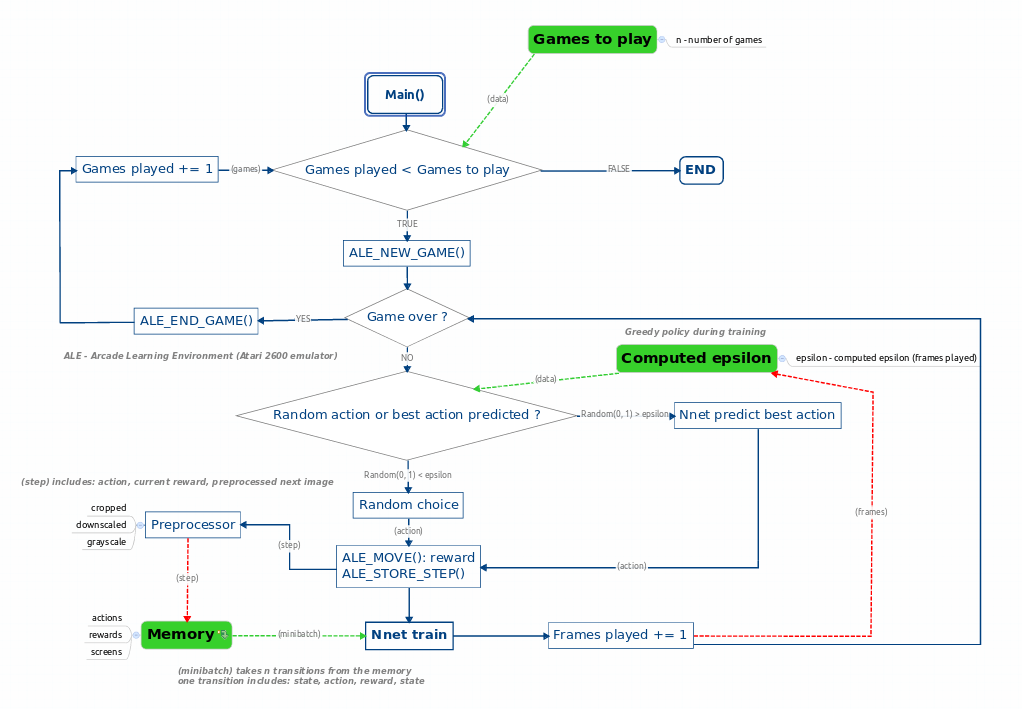
\includegraphics[scale=0.38]{flow.png}
    \caption{Implementation algorithm}
    \label{fig:imp_algo}
\end{figure}

Implementation of the memory model is relatively simple (Figure \ref{fig:mem_model}).
\begin{figure}[h]
    \centering
    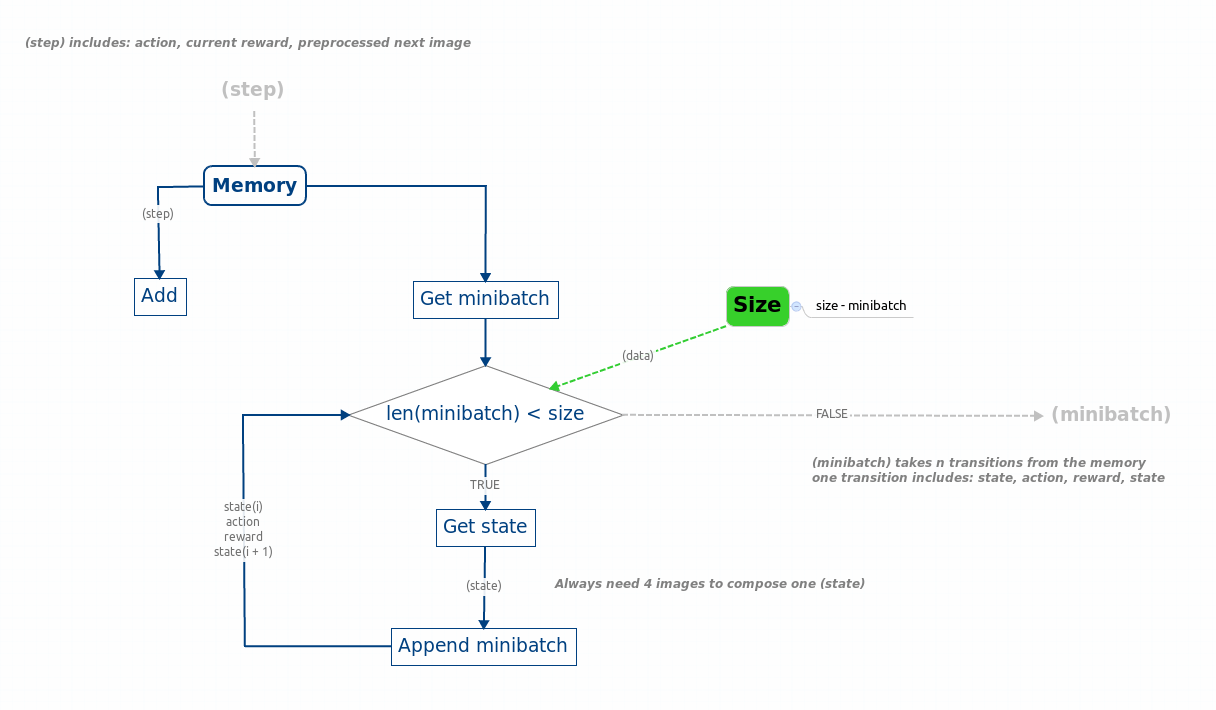
\includegraphics[scale=0.29]{memory_model.png}
    \caption{Memory model}
    \label{fig:mem_model}
\end{figure}

\subsection[Wrappers]{Wrappers}

Our library (DRL) provides a set of wrappers, each of these connects to appropriate game environment (Atari, Nintendo and others) using available software interfaces. The wrapper interacts with environment by sending it a commands to perform an actions or to obtain the necessary information about environment internal state (such as game reward, termination state etc). It also receives a video output from environment and processes it sequentially as an image stream. The wrapper is the only game-specific and non-generalized component in our solution. General diagram of DSG technology stack is provided on Figure \ref{fig:tech_stack}.

\subsubsection[List of the supported wrappers]{List of the supported wrappers}
\label{sec:wrappersList}
\begin{center}
    \begin{tabu}{ | c | c | c | c | p{2.5cm} | p{5cm} |}
    \hline
    \rowfont{\bfseries}
    \textbf{Name} & \textbf{Type} & \textbf{Interface} & \textbf{Python class} & \textbf{Environments} & \textbf{Description} \\ \hline
    \rowfont{\scriptsize}
    atari & Emulator & FIFO (text file) & ale.ALE
    & \noindent
    \begin{itemize}[noitemsep,topsep=0pt,parsep=0pt,partopsep=0pt]
        \item Breakout
        \item Space Invaders
    \end{itemize}
    & The Arcade Learning Environment (ALE) is a simple object-oriented framework that allows to develop AI agents for Atari 2600 games
    \footnote{\url{http://www.arcadelearningenvironment.org/}}. \\
    \hline
    \end{tabu}
\end{center}

\subsection[TNNF Framework]{TNNF Framework}
Our Deep Learning implementation is based on TNNF framework which is also developed by our group. Please refer to the project documentation page \footnote{\url{http://tnnf.readthedocs.org/en/latest}} to get further information.
\begin{figure}[h]
    \centering
    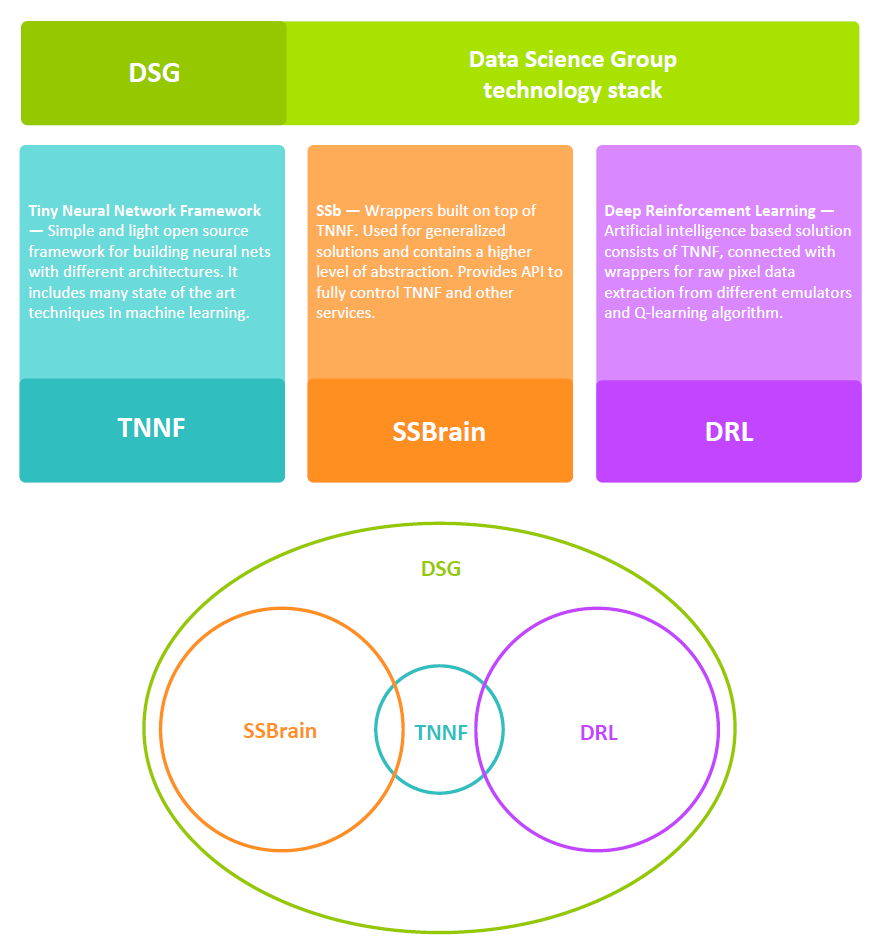
\includegraphics[scale=0.53]{DSG_tech_stack.png}
    \caption{DSG technology stack}
    \label{fig:tech_stack}
\end{figure}

\subsection[GPU Computing]{GPU Computing}
\label{sec:gpuComputing}
Great progress achieved in last 10 years in the area of general-purpose computing on GPUs
\footnote{\url{http://en.wikipedia.org/wiki/General-purpose\_computing\_on\_graphics\_processing\_units}}
\footnote{\url{http://www.nvidia.com/object/what-is-gpu-computing.html}}
also brought a great benefit to the field of Artificial Intelligence (and to the Deep Learning in particular
\footnote{\url{http://devblogs.nvidia.com/parallelforall/accelerate-machine-learning-cudnn-deep-neural-network-library/}}
) since its incredible ability to massively parallel computation provides an exponential increase in performance (up to 50 times faster) on linear algebra operations that are so resource intensive with traditional CPU-based approach, especially on a large datasets.\\\\
There are two main frameworks that implements this computational model:
\begin{itemize}
    \item NVIDIA CUDA (proprietary)
    \footnote{\url{http://en.wikipedia.org/wiki/CUDA}}
    \item OpenCL (open source)
    \footnote{\url{http://en.wikipedia.org/wiki/OpenCL}}
    \\
\end{itemize}
The neural network framework (TNNF) we use in this project, is built on the top of the Theano library
\footnote{\url{http://deeplearning.net/software/theano/}}
which in turn uses CUDA to perform GPU-based computations. Please refer to the project documentation
\footnote{\url{http://deeplearning.net/software/theano/tutorial/using\_gpu.html}}
for more information on how to install and configure CUDA-backend in case if your GPU device is supported by vendor
\footnote{\url{http://en.wikipedia.org/wiki/CUDA\#Supported_GPUs}}.\\\\
Our solution uses all advantages of this approach, however it still could be used in a traditional way of CPU computing (see \hyperref[sec:config]{Configuration})


\subsection[MDP Environment]{MDP Environment}
In our project, we consider the following MDP environment $\varepsilon$:
\begin{itemize}
    \item Raw screen images from the game video output represent $s \in S$;
    \item Available game actions obviously represent set $A = \{a_1,\dots,a_k\}$;
    \item Game reward obtained through API represents $r_t$;
\end{itemize}

\subsection[Preprocessing]{Preprocessing}
We perform a basic preprocessing step on each of raw $210 \times 160$ RGB images from input video stream. It consists:
\begin{itemize}
    \item cropping a square $160 \times 160$ region of original image;
    \item downscaling to $84 \times 84$ image;
    \item converting RGB to gray-scale or B/W representation;
\end{itemize}

\subsection[Neural Network]{Neural Network}
We use a Neural Network in conjunction with advanced Deep Learning techniques as a action-value function approximator. We refer to it as a DRL-network with weights $\theta$ which estimates $Q(s,a;\theta)$.

\subsubsection[Network topology]{Network topology}
DRL-network architecture consists of the following layers:
\newpage
\begin{enumerate}
% \begin{enumerate}[noitemsep,topsep=0pt,parsep=0pt,partopsep=0pt]
    \item Input layer (L1)
        \begin{itemize}
            \item Layer type: Convolutional
            \item Activation function: Leaky Rectified Linear Unit \footnote{\url{http://en.wikipedia.org/wiki/Rectifier\_(neural_networks)\#Leaky\_ReLUs}}
            \item Number of inputs: $28224$
            \item Number of outputs: $6400$
            \item Convolutional filter shape: $16 \times 4 \times 8 \times 8$
        \end{itemize}
    \item Hidden layer (L2)
        \begin{itemize}
            \item Layer type: Convolutional
            \item Activation function: Leaky Rectified Linear Unit
            \item Number of inputs: $6400$
            \item Number of outputs: $2592$
            \item Convolutional filter shape: $32 \times 16 \times 4 \times 4$
        \end{itemize}
    \item Hidden layer (L3)
        \begin{itemize}
            \item Layer type: Fully connected
            \item Activation function: Rectified Linear Unit \footnote{\url{http://en.wikipedia.org/wiki/Rectifier\_(neural_networks)}}
            \item Number of inputs: $2592$
            \item Number of outputs: $256$
        \end{itemize}
    \item Output layer (L4)
        \begin{itemize}
            \item Layer type: Fully connected
            \item Activation function: Linear function
            \item Number of inputs: $256$
            \item Number of outputs: \textit{depends on a number of actions in particular game environment}
        \end{itemize}
\end{enumerate}
\begin{figure}[h]
    \centering
    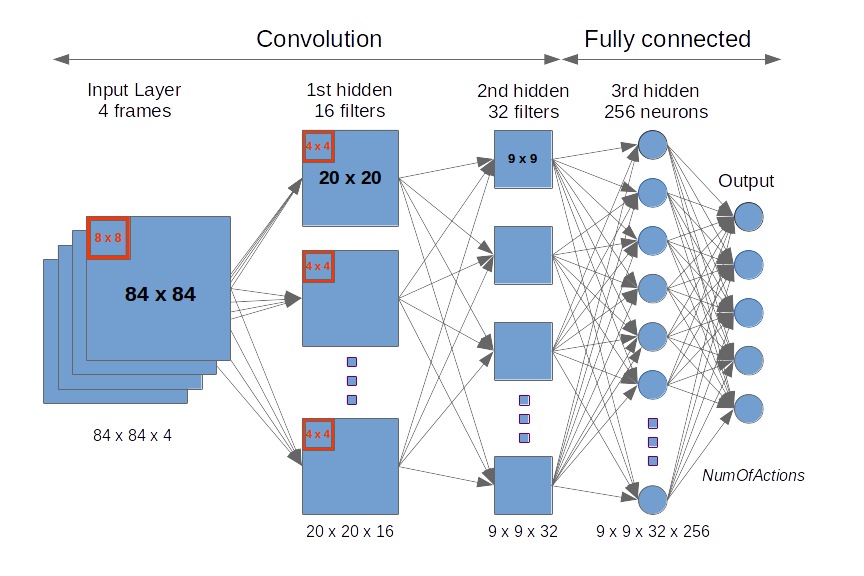
\includegraphics[scale=0.50]{ss_nn_schm.png}
    \caption{DRL Neural Network}
    \label{fig:neural_net}
\end{figure}

\subsubsection[Network model]{Network model}
The following functions are used:

\begin{equation}
C_{p}^{'}(i,j) = ln(1 + exp(\sum_{z=-3}^{4}\sum_{v=-3}^{4}(h_{pzv}^{'} \times S_{u}(2(i-3)+1+z,2(j-3)+1+z))))
\end{equation}

\begin{equation}
C_{t}^{''}(i,j) = ln(1 + max(\sum_{z=-1}^{2}\sum_{v=-1}^{2}(h_{tzv}^{''} \times C_{p}^{'}(2(i-1)+1+z,2(j-1)+1+z)),0))
\end{equation}

\begin{equation}
F_{k} = ln(1 + max(\sum_{t=1}^{32}\sum_{i=1}^{9}\sum_{j=1}^{9}(w_{tijk}^{C} \times C_{t}^{''}(i,j)),0))
\end{equation}

\begin{equation}
Q_{r} = \sum_{k=1}^{256}(w_{kr}^{F} \times F_{k})
\end{equation}
where

\begin{equation}
t = (p-1) \times 2 + q_{2}; \quad
p = (u-1) \times 4 + q_{1}; \quad
q_{1} = \overline{1,4}; \quad
q_{2} = \overline{1,2}; \quad 
u = \overline{1,4}
\end{equation}
S --- input layer images \\
$C^{'}$ --- first convolutional layer images \\
$C^{''}$ --- second convolutional layer images \\
F --- hidden fully connected layer \\
Q --- output layer

\subsubsection[Training]{Training}
A DRL-network is trained by minimizing a loss functions $L_i (\theta_i)$ on each iteration $i$, using RMSProp algorithm with mini-batches of size 128 samples:
\begin{equation} \label{eq:activation}
    L_i(\theta_i) = (y_i - Q(s,a,\theta_i))^2
\end{equation}
Here, $y = \mathbb{E}_{s'\sim \varepsilon}[r + \gamma \max_{a'} Q(s', a';\theta_{i-1})|s,a]$ is the target return for iteration $i$.\\
\\
Differentiating the loss function with respect to the weights we get the following gradient:
\begin{equation} \label{eq:activation}
    \nabla_{\theta_i} L_i(\theta_i) = \Big[r + \gamma \max_{a'} Q(s', a';\theta_{i-1}) - Q(s,a,\theta_i)\Big]\nabla_{\theta_i} Q(s,a,\theta_i)
\end{equation}
\\
In terms of MDP, on each time-step $t$ in states $s_t,s_{t+1}'$ we divide environment timeline (Figure \ref{fig:states}) into following parts:
\begin{itemize}
    \item Pre-state - set of the last 4 image before state $s_t$;
    \item Post-state - set of the last 4 image before state $s_{t+1}'$, when an action $a_t$ has already been applied;
\end{itemize}
\begin{figure}[H]
    \centering
    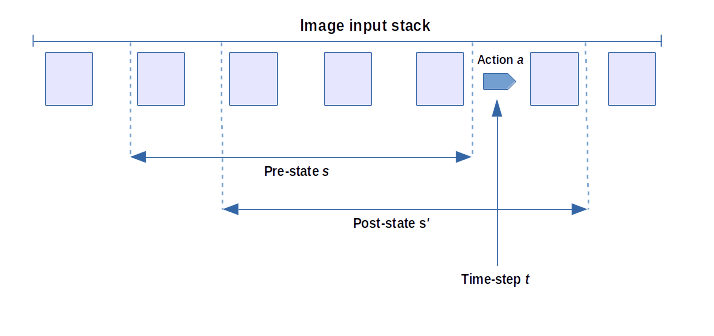
\includegraphics[scale=0.50]{states.png}
    \caption{Timeline illustration}
    \label{fig:states}
\end{figure}
On each game iteration $i$, agent receives from environment wrapper a pre-state sequence $s$. Then it selects an action to be performed by following an $\epsilon$-greedy strategy and using DRL-network to estimate $\max_{a} Q(s, a;\theta_i)$. Subsequently agent moves into post-state $s'$ and gets a reward $r$. Reward takes value from set \{-1,0,1\}, where
\begin{itemize}[noitemsep]
	\item 1 - success (ball broke the brick)
	\item 0 - no action is required
	\item -1 - failure (ball was lost)
\end{itemize} 
The sequence (s, a, r, s') forms a transition unit and is used to train DRL-network by estimating $y = \mathbb{E}_{s'\sim \varepsilon}[r + \gamma \max_{a'} Q(s', a';\theta_{i-1})|s,a]$. Complete training process workflow is reflected on Figure \ref{fig:a_workflow}.
\begin{figure}[H]
    \centering
    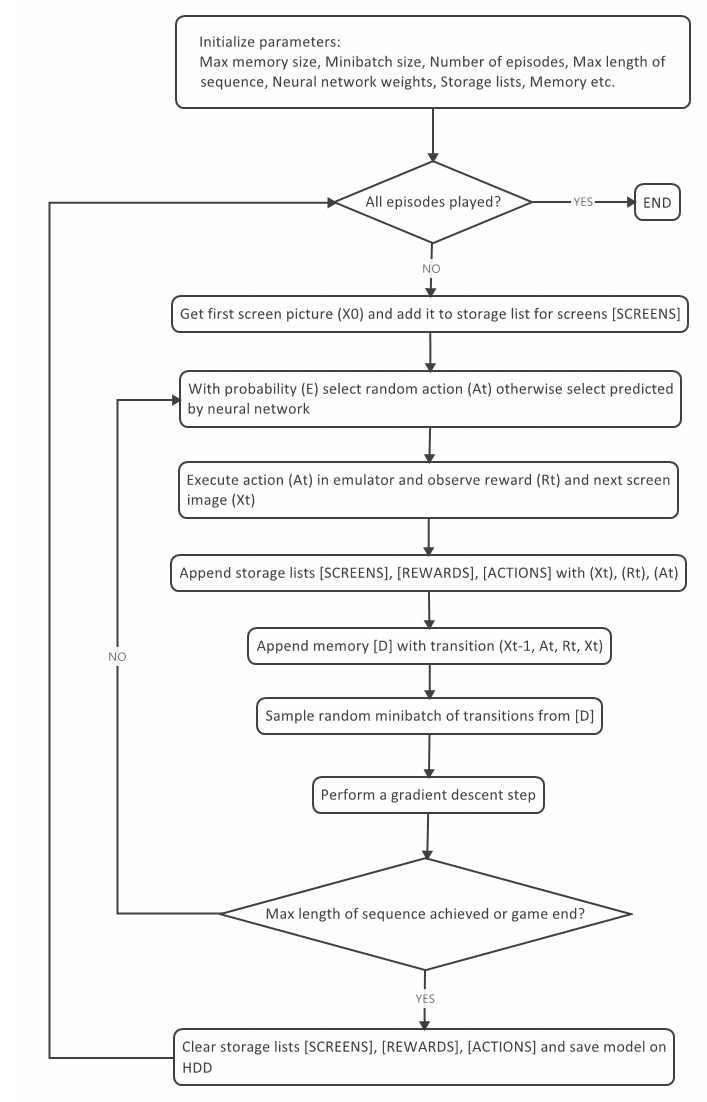
\includegraphics[scale=0.40]{alorithm.png}
    \caption{Complete workflow}
    \label{fig:a_workflow}
\end{figure}

\subsection[Further improvements]{Further improvements}
\label{subsec:improvements}

There still exist, many possible options for our algorithm’s improvement:
\begin{enumerate}
\item Initialization of connection weights to C-layers, based on preliminary analysis of the controlled object. We can assume that the convulsion kernels, which were got after neural network training finishing, reduce to the set of “lines” and “spots” filters, so if the initialization was performed based on  pre-set filters, it could significantly decrease required training time.
\item Network architecture can be extended by recurrent layer, for providing the possibility to get clustering of  video series with  unlimited number of clusters. This network can be trained to recognize the new information without retraining. This approach allows to generalize input information and use the optimal solution in the case, when we get new image (video series), but which is referred to the known class.
\item Sparsity helps extract better features from raw data, more complex and generalized.
\footnote{\url{http://ufldl.stanford.edu/wiki/index.php/Autoencoders_and_Sparsity}}
\item After obtaining features using convolution, we would next like to use them for classification. In theory, one could use all the extracted features with a classifier such as a softmax classifier, but this can be computationally challenging. To address this we could use aggregation operation called pooling.
\footnote{\url{http://ufldl.stanford.edu/wiki/index.php/Pooling}}
\item Dropout as universal regularization works better than weight decay and fix the overfitting problem.
\footnote{\url{http://jmlr.org/papers/volume15/srivastava14a/srivastava14a.pdf}}
\item Long short term memory (LSTM), which is a recurrent neural network (RNN) architecture, can be used instead of experience replay technique.
\footnote{\url{http://en.wikipedia.org/wiki/Long_short_term_memory}}
\end{enumerate}

\section[Getting Started with DRL]{Getting Started with DRL}
\label{sec:gettingStarted}
Questions, that are covered in this section: 
\begin{itemize}
  \item Installing all needed packages for project to run;
  \item Getting DRL source code and preparing for launching the training process;
  \item Structure of the project;
  \item Advance fitting.
\end{itemize}
All actions should be performed using the command line. Please, perform the next steps to launch terminal emulator in Ubuntu 14.04 or CentOS 7 (supported systems in this guide):
\begin{itemize}
  \item Ubuntu 14.04 \\
  Press the \textbf{Alt-Ctrl-T} shortcut or use the graphic interface: press \textbf{Win}, then type ``term'' and choose your favorite:
  \begin{figure}[H]
    \centering
    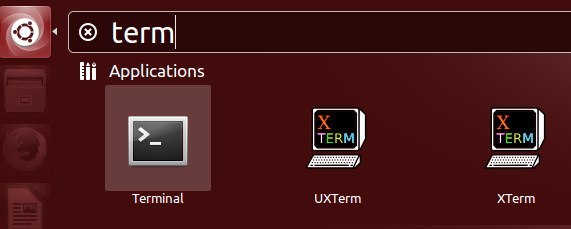
\includegraphics[width=0.6\textwidth]{terminal.png}
    \caption*{Starting terminal using GUI in Ubuntu}
    \label{fig:UbuntuTerm}
  \end{figure}
  \item CentOS 7 \\
  In CentOS there is no hotkey to start the terminal. But there is two ways to start it using GUI:
    \subitem Using ``Application'' menu:
    \begin{figure}[H]
      \centering
 
      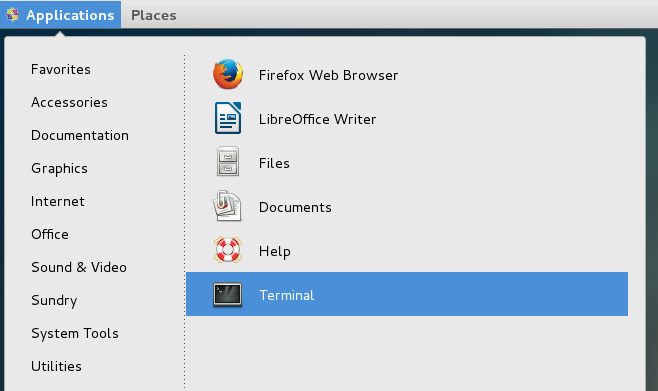
\includegraphics[width=0.6\textwidth]{centos_term.png}
      \caption*{Starting terminal using GUI in CentOS with Application menu}
      \label{fig:CentosTerm}
    \end{figure}
    \subitem Using \textbf{Win} button: press \textbf{Win}, then type ``term'' and choose your favourite
    \begin{figure}[H]
      \centering
      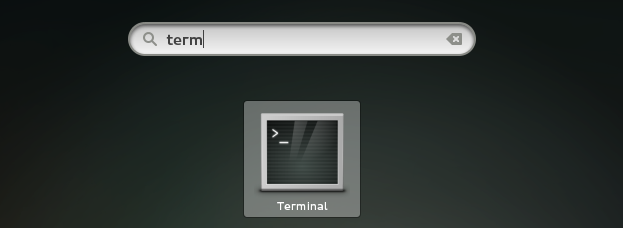
\includegraphics[width=0.6\textwidth]{centos_win_term.png}
      \caption*{Starting terminal using GUI in CentOS with Win button}
      \label{fig:CentosTermWin}
    \end{figure}


\end{itemize}
\subsection[Requirements]{Requirements}
\begin{tcolorbox}[colbacktitle=red!40!white, coltitle=black, width=\linewidth, fonttitle=\bfseries, title=Note]
Please check the following requirements before you start an installation.
\end{tcolorbox}
\noindent
Supported operating systems (desktop versions):
\begin{itemize}
\item CentOS 7
  \footnote{\url{http://www.centos.org/download}}
\item Ubuntu 14.04
  \footnote{\url{http://www.ubuntu.com/desktop}}
\end{itemize}
Hardware requirements:
\begin{itemize}
\item \textbf{CPU}: 64-bit Intel or AMD multi-core processor (2+ Cores)
\item \textbf{RAM}: 8GB of RAM (16GB recommended)
\item \textbf{GPU}: CUDA supported video card 
  \footnote{\url{https://developer.nvidia.com/cuda-gpus}}
\item \textbf{Disk Space}: 8GB of free disk space
\end{itemize}
Make sure that your user is able to sudo. Run in terminal this command to do it:
\begin{minted}{bash}
sudo -l
\end{minted}
\noindent
The output should be like following:
\begin{tcolorbox}[colbacktitle=gray!40!white, coltitle=black, width=\linewidth, fonttitle=\bfseries, title=Output]
User <user> may run the following commands on <host>:

(ALL : ALL) ALL
\end{tcolorbox}
\begin{figure}[H]
  \centering
  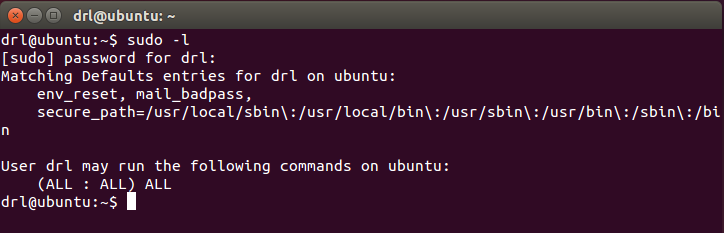
\includegraphics[width=1\textwidth]{sudo_access.png}
  \caption*{Check sudo access}
  \label{fig:sudoAccess}
\end{figure}
\noindent
If there is an error in the output, please ask your system administrator to provide you appropriate sudo rights. \footnote{\url{http://www.pendrivelinux.com/how-to-add-a-user-to-the-sudoers-list/}}



\subsection[Virtual Machine]{Virtual Machine}
For your convenience, we prepared a virtual machine image (in OVA format) containing fully operative demonstration setup of the DRL. With this image you would be able to test the pre-trained model, but without training, so you don't need CUDA supported video card and 4GB of RAM is enough. \\

\begin{tcolorbox}[colbacktitle=red!40!white, coltitle=black, width=\linewidth, fonttitle=\bfseries, title=Note]
Demonstration build can be used only with a traditional CPU-based approach, since it is currently impossible to emulate a NVIDIA environment.
\end{tcolorbox}

\noindent
\\ There are two distributions available in a Download section on a project web page:
\begin{itemize}
    \item CentOS based
    \item Ubuntu Linux based
\end{itemize}

\noindent
\\ After extracting an image from archive, follow the instructions below:
\begin{enumerate}
    \item Import an extracted VM image into your virtual environment (VMware Player, VirtualBox etc.);
    \item Configure an instance according to the hardware requirements;
    \item Start an instance;
    \item Access to the virtual machine console and log into a desktop environment using following credentials:
        \begin{itemize}
            \item Login: drl
            \item Password: admin
        \end{itemize}
    \item Open the README file on the Desktop;
    \item Follow the instructions in README.
\end{enumerate}

\noindent
Now you can test the pre-trained model. If you want to train a model by yourself, follow the instructions in the following sections.



\subsection[Installation]{Installation}

Installation process was tested on supported systems (CentOS 7 and Ubuntu 14.04) installed on virtual machines from the official sites. Before installation there wasn't any additional software except for software, that was provided with this distributives.

In this section will be covered questions about what packages are needed for DRL to work properly and how to install them.

\subsubsection[Needed packages]{Needed packages}
See ``How to install'' section (\ref{installation}) to perform installation of this libraries.

Names of packages are provided in format: 
\begin{tcolorbox}[colbacktitle=gray!40!white, coltitle=black, width=\linewidth, fonttitle=\bfseries, title=Conventions]
<Ubuntu\_package>/<CentOS\_package> - names of packages in both supported systems delimited by slash (/)
\end{tcolorbox}
OR
\begin{tcolorbox}[colbacktitle=gray!40!white, coltitle=black, width=\linewidth, fonttitle=\bfseries, title=Conventions]
<Name\_of\_package> (System) - if package is needed to be installed only 
\end{tcolorbox}

\paragraph*{General purpose packages:}

\begin{itemize}
  \item \textit{g++/gcc-c++} - the C++ front end for GCC compiler.
  \item \textit{libopenblas-dev/blas-devel} - The BLAS (Basic Linear Algebra Subprograms) are routines that provide standard building blocks for performing basic vector and matrix operations. 
    \footnote{\url{http://www.netlib.org/blas/}}
  \item \textit{libyaml-dev/libyaml-dev} - YAML is a human friendly data serialization standard for all programming languages. Is needed for pylearn2. 
    \footnote{\url{http://www.yaml.org}}
  \item SDL packages:
\\
\subitem \textit{libsdl1.2-dev/SDL-devel.x86\_64}
\subitem \textit{libsdl-image1.2-dev/SDL\_image-devel.x86\_64}
\subitem \textit{libsdl-gfx1.2-dev/SDL\_gfx-devel.x86\_64}
\\

    SDL - Simple DirectMedia Layer is a cross-platform development library designed to provide low level access to audio, keyboard, mouse, joystick, and graphics hardware via OpenGL and Direct3D. It is used by video playback software, emulators, and popular games. 
    \footnote{\url{https://www.libsdl.org/}}
  \item \textit{gcc (CentOS)} - compiler system produced by the GNU Project supporting various programming languages. 
    \footnote{\url{https://gcc.gnu.org/}}
  \item \textit{gcc-gfortran (CentOS)} - free Fortran 95/2003/2008 compiler for GCC. 
    \footnote{\url{https://gcc.gnu.org/wiki/GFortran}}
  \item \textit{lapack-devel (CentOS)} - provides routines for solving systems of simultaneous linear equations, least-squares solutions of linear systems of equations, eigenvalue problems, and singular value problems. 
    \footnote{\url{http://www.netlib.org/lapack/}}
  \item \textit{atlas-devel (CentOS)} - provides C and Fortran77 interfaces to a portably efficient BLAS implementation. 
    \footnote{\url{http://math-atlas.sourceforge.net/}}
  \item \textit{zlib-devel.x86\_64 (CentOS)} - general purpose compression library. 
    \footnote{\url{http://www.zlib.net/}}
\end{itemize}

\paragraph*{Python packages:}\mbox{}\\
This section is about what packages should be installed before DRL installation. The common commands for installation of this packages you can find in the next section. This information is provided for you to be informed what libraries do DRL use.
Some of this packages need to be installed using \textbf{pip}. To find out which tool to use - see the next section.

\subparagraph*{List of packages:}
\begin{itemize}
  \item \textit{python-dev/python-devel} - contains the header files and libraries needed for python to be extended with dynamically loaded extensions. 
    \footnote{\url{https://www.python.org/}}
  \item \textit{python-pip/pip} - recommended tool for installing Python packages. 
    \footnote{\url{https://pypi.python.org/pypi/pip/}}
  \item \textit{python-numpy/numpy==1.6.1} - the fundamental package for scientific computing with Python. 
    \footnote{\url{http://www.numpy.org/}}
  \item \textit{python-scipy/scipy==0.10.1} - Python-based ecosystem of open-source software for mathematics, science, and engineering. 
    \footnote{\url{http://www.scipy.org/}}
  \item \textit{python-matplotlib/python-matplotlib} - Python 2D plotting library. 
    \footnote{\url{http://matplotlib.org/}}
  \item \textit{Theano/Theano} - a Python library that allows you to define, optimize, and evaluate mathematical expressions involving multi-dimensional arrays efficiently. 
    \footnote{\url{http://deeplearning.net/software/theano/}}
  \item \textit{pylearn2/pylearn2} - machine learning library. Needed in DRL for Convolution Networks. 
    \footnote{\url{https://github.com/lisa-lab/pylearn2}}
  \item \textit{python-pil/python-pillow} - Python imaging library. 
    \footnote{\url{http://www.pythonware.com/products/pil/}}
  \item \textit{python-nose/python-nose} - testing library for Python. 
    \footnote{\url{https://nose.readthedocs.org/en/latest/}}
\end{itemize}

\subsubsection[How to install]{How to install}
\label{installation}
DRL is written in Python, so make sure that you have at Python 2.7 or later installed on your system. It may be easily checked from the command line:
\begin{minted}{bash}
python --version
\end{minted}
\begin{figure}[H]
  \centering
  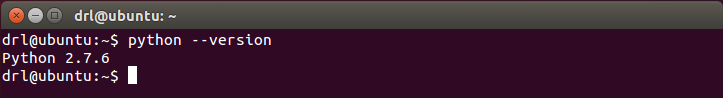
\includegraphics[width=1\textwidth]{python_version.png}
  \caption*{Check Python version}
  \label{fig:pythonVersion}
\end{figure}
If the output looks like \textit{``Python 2.7.x''} (Python 3.x.x is not ok) - you have the correct version of Python and you can skip Python installation section. In case of error or another version, please, install the correct version of Python on your system and, if needed, make a symlink \textit{``python''} in one of the \$PATH directories to the interpreter of this version.

\paragraph*{Python installation:}
\begin{itemize}
\item Ubuntu 14.04:
\begin{minted}{bash}
sudo apt-get install build-essential
sudo apt-get install libreadline-gplv2-dev libncursesw5-dev libssl-dev \
libsqlite3-dev tk-dev libgdbm-dev libc6-dev libbz2-dev
cd ~/Downloads/
wget http://python.org/ftp/python/2.7.5/Python-2.7.5.tgz
tar -xvf Python-2.7.5.tgz
cd Python-2.7.5
./configure
make
sudo make install
\end{minted}

\noindent
\item CentOS 7:
\begin{minted}{bash}
sudo yum groupinstall "Development tools"
sudo yum install zlib-devel bzip2-devel openssl-devel ncurses-devel \
sqlite-devel readline-devel tk-devel gdbm-devel db4-devel libpcap-devel \
xz-devel
cd ~/Downloads/
wget --no-check-certificate \
https://www.python.org/ftp/python/2.7.5/Python-2.7.5.tar.xz
tar -xvf Python-2.7.5.tar.xz
cd Python-2.7.5
./configure --prefix=/usr/local
make 
sudo make altinstall
\end{minted}
\end{itemize}

\paragraph*{Pre-installation:}\mbox{}\\
If you are using CentOS, you should add \textit{EPEL} and \textit{RPMForge} repositories:
\begin{minted}{bash}
sudo yum install \
http://dl.fedoraproject.org/pub/epel/7/x86_64/e/epel-release-7-5.noarch.rpm
sudo yum install \
http://pkgs.repoforge.org/rpmforge-release/rpmforge-release-0.5.3-1.el7.rf.x86_64.rpm
\end{minted}

\noindent
Paste following lines line by line to your terminal to install all needed packages:
\begin{itemize}
\item Ubuntu 14.04:
\begin{minted}{bash}
sudo apt-get install python-pil python-numpy python-scipy python-dev \
python-pip python-nose g++ libopenblas-dev git libsdl1.2-dev \
libsdl-image1.2-dev libsdl-gfx1.2-dev python-matplotlib libyaml-dev
sudo pip install -U numpy
sudo pip install -U pillow==2.7.0
sudo pip install Theano
\end{minted}
\item CentOS 7:
\begin{minted}{bash}
sudo yum install python-devel python-nose python-pillow python-setuptools \
gcc gcc-gfortran gcc-c++ blas-devel lapack-devel atlas-devel \
SDL-devel.x86_64 SDL_image-devel.x86_64 SDL_gfx-devel.x86_64 \
zlib-devel.x86_64 git python-matplotlib libyaml-dev
sudo easy_install pip
sudo pip install -U numpy
sudo pip install -U pillow==2.7.0
sudo pip install scipy
sudo pip install Theano
\end{minted}
\end{itemize}

Also, you should install \textit{pylearn2} package. Steps are the same for the both systems:
\begin{minted}{bash}
cd ~/ # Or any other directory where you want the pylearn2 project to be stored
git clone https://github.com/lisa-lab/pylearn2.git
cd ./pylearn2
sudo python setup.py develop
\end{minted}

DRL project is developed and tested with CUDA (parallel computing platform and programming model created by NVIDIA\footnote{\url{https://developer.nvidia.com/cuda-zone}}). CUDA is developed for fast GPU computing. CPU mode is also available, but deep reinforcement learning in this mode is too slow, so CPU mode is not recommended for learning. However, if you have a trained model, it is possible to test it on CPU without any speed issues. \\
\indent
Follow the instructions on NVIDIA page to install CUDA SDK\footnote{\url{http://docs.nvidia.com/cuda/cuda-getting-started-guide-for-linux/index.html\#pre-installation-actions}}. \\
\indent
Also, if you want to use CUDA not only in this terminal session, you have to change some global variables in your \textit{\raisebox{0.5ex}{\texttildelow}/.bashrc}:
\begin{minted}{bash}
cat >> ~/.bashrc <<EOF
export PATH=/usr/local/cuda-6.5/bin:$PATH
export LD_LIBRARY_PATH=/usr/local/cuda-6.5/lib64:$LD_LIBRARY_PATH
EOF
\end{minted}

Great! You system is ready for DRL to be installed and tested.

\paragraph*{DRL installation:}\mbox{}\\

To install DRL you need to:
\begin{enumerate}
\item Make sure that correct Python version is installed in your system and Python interpreter can by started with ``python'' command.
\item Make all the pre-installation steps. Make sure that everything is installed properly without errors.
\item Clone source code from GitHub\footnote{\url{https://github.com/DSG-SoftServe/DRL}}:
\begin{minted}{bash}
git clone https://github.com/DSG-SoftServe/DRL
\end{minted}
\item Navigate to the project directory
\begin{minted}{bash}
cd DRL
\end{minted}
\item Run \textit{install.sh} script.
\begin{minted}{bash}
bash ./install.sh
sudo chown -R $USER ~/.theano # to run the demo without sudo
\end{minted}
\end{enumerate}

If installation is succeed, the environment is ready to use.

\subsubsection[CPU mode]{CPU mode}
It is not recommended to run the demo in CPU mode. But, if you don't have NVIDIA GPU and want to check out if it's working, apply this fix:
\begin{minted}{bash}
cd src
drl_optimize=False # False for CPU, True for GPU
drl_regex="(\s*optimized=)[a-zA-Z]+(\))"
sed -ri "s:$drl_regex:\1$drl_optimize\2:g" ai/neuralnet.py
\end{minted}

\begin{tcolorbox}[colbacktitle=red!40!white, coltitle=black, width=\linewidth, fonttitle=\bfseries, title=WARNING]
Use only "False" and "True" values
\end{tcolorbox}

To launch the demo in CPU mode, use \textit{"cpuRun.sh"} instead of \textit{"gpuRun.sh"} in future paragraphs.

\subsection[Launching and using]{Launching and using}
\subsubsection{First launch}
You have DRL installed and it's time for the first launch. \\
Navigate to the DRL project directory and perform following steps to launch the learning process:
\begin{minted}{bash}
cd ./src/
bash gpuRun.sh main_exp.py
\end{minted}

Congratulations, you have launched the deep reinforcement learning process. \\
Now you should see the window like this:
\begin{figure}[h]
    \centering
    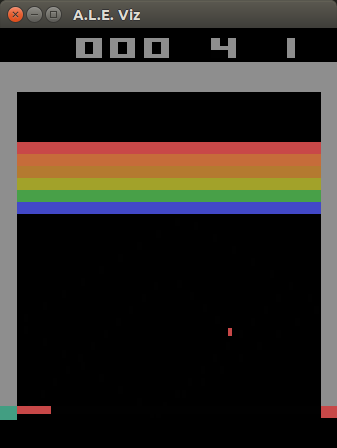
\includegraphics[scale=0.53]{breakout.png}
    \caption{Breakout}
    \label{fig:theGame}
\end{figure}

Also, there should be an output in the command line like this:
\begin{tcolorbox}[colbacktitle=gray!40!white, coltitle=black, width=\linewidth, fonttitle=\bfseries, title=Output]
action RAND: 2 \\
S: 50 A: 49 R: 49 D: 171 \\
\_\_\_\_\_\_\_\_\_\_ Reward  0 \\
Step: 177 \\
0.04417 
\end{tcolorbox}

Let's find out what does this indicators means:
\begin{itemize}
    \item \textit{action RAND: 2} - there is 4 available actions ([0..3]). The action can be chosen from neural network (NN) experience with probability $\epsilon$, where 0<$\epsilon$<1. Than you'll see ``NEURALNET'' instead of ``RAND''. Otherwise, NN will perform a random action;
    \item \textit{S: 50} - current state. States are changing with ascending order starting from 0 since last negative reward;
    \item \textit{A: 49} - performed action. Logic of numbering is similar to state;
    \item \textit{R: 49} - reward for action. Logic of numbering is similar to state;
    \item \textit{D: 171} - memory;
    \item \textit{Reward 0} - current value of reward. Could be -1, 0 or 1;
    \item \textit{Step: 177} - number of steps performed from the learning start;
    \item \textit{0.04417} - time, spent for the step (in minutes).
\end{itemize}

\noindent
``S'', ``A'' and ``R'' are from the Markov decision processes (MDPs) model\footnote{\url{http://en.wikipedia.org/wiki/Markov_decision_process}}. \\
\noindent
So, we can see such correlations between command line and window:
\begin{itemize}
    \item when the ``action'' is changing, the actor (bottom block) changes it's behavior;
    \item when the shell hits one of the upper blocks, the reward equals 1;
    \item when the actor looses the last life, the reward equals -1.
\end{itemize}

\subsubsection{Project structure}
Let's look closer at some of the important parts of the project. Below, you can see the output of Unix ``tree -d'' command, except for unnecessary for understanding folders:
\mbox{}\\
\mbox{}\\
\begin{tikzpicture}[%
  grow via three points={one child at (0.5,-0.7) and
  two children at (0.5,-0.7) and (0.5,-1.4)},
  edge from parent path={(\tikzparentnode.south) |- (\tikzchildnode.west)}]
  \node [selected]{DRL}
    child { node {libraries}
      child { node {ale}
        child { node {doc}}
        child { node {roms}}
        child { node {src}}
        child { node {state}}
      }
    }
    child [missing] {}        
    child [missing] {}        
    child [missing] {}
    child [missing] {}
    child [missing] {
    }       
    child { node {src}
      child { node {ai}}
      child { node {ale}}
      child { node {data}}
      child { node {graphs}}
      child { node {memory}}
      child { node {models}}
      child { node {tnnf}}
    };
\end{tikzpicture}
\mbox{}\\

There is two folders in the root of the project structure that need to be mentioned:
\begin{itemize}
\item \textbf{libraries} - contains \textit{``ale''} folder. ALE is a tool, which gave the ability to learn models on different Atari games. From the official site: \\
  The Arcade Learning Environment (ALE) is a simple object-oriented framework that allows researchers and hobbyists to develop AI agents for Atari 2600 games. It is built on top of the Atari 2600 emulator Stella and separates the details of emulation from agent design. 
  \footnote{\url{http://www.arcadelearningenvironment.org/}}
The most interesting folder in libraries/ale directory is roms. Here you can find games, for which you can train NN. (see the additional fitting chapter)
\item \textbf{src} - the main folder obviously. All source code of the DRL project is located in this folder.
Five directories should be mentioned here:
\subitem \textit{ai} - source code of neural network, which is used within the project;
\subitem \textit{ale} - wrapper code for interaction with the Arcade Learning Environment;
\subitem \textit{data} - scripts to work with data;
\subitem \textit{graphs} - graphs with experiment results;
\subitem \textit{memory} - implementation of neural network memory;
\subitem \textit{models} - directory, where all trained models will be located;
\subitem \textit{tnnf} - source code for Tiny Neural Net Framework.
  \footnote{\url{http://tnnf.readthedocs.org/en/latest/index.html}}
  used to create and train the neural network, which is used in this project.
\end{itemize}

The \textbf{graphs} directory contains following graphs:
\begin{itemize}
\item \textit{rewargs.png} - sum of rewards for multiple iterations (1000 by default), e.g. Left plots on Figures \ref{fig:random} and \ref{fig:trained};
\item \textit{rgstat.png} - average rewards for 1 finished game from multiple iterations (1000 by default), e.g. Right plots on Figures \ref{fig:random} and \ref{fig:trained};
\item \textit{wsum.png} - sum of the weights on both convolutional layers of neural network.
\end{itemize}

\subsubsection[Using existing models]{Using existing models}
The result of the training part is a file, saved in \textit{DRL/src/models/} directory. You can use this file to find out how good your NN was trained. You can use the \textit{play.py} script in the \textit{src} directory to play a game with your trained NN. Launching game with a trained NN is similar to training launching:
\begin{minted}{bash}
cd DRL/src
bash gpuRun.sh play.py
\end{minted}

You should see the similar to the training output: window with the game and output in command line. But there shouldn't be any training time in the output.

In the first version of DRL there is no ways to configure which model to use, except for editing \textit{play.py} script. By default, the pre-trained model ``\raisebox{0.5ex}{\texttildelow}\raisebox{0.5ex}{\texttildelow}p-AS.model.weights.NN.NMem.906508'' is hardcoded.

You can change the script to use your own model in two ways: to edit the file or to run the \textit{sed} tool.

\begin{tcolorbox}[colbacktitle=red!40!white, coltitle=black, width=\linewidth, fonttitle=\bfseries, title=Note]
path to the model is relative to the play.py script
\end{tcolorbox}

\paragraph*{Edit the file using text editor}
\begin{enumerate}
\item In command line navigate to the DRL project directory, then to \textit{src} folder. Using your favorite text editor, open the \textit{play.py} script;
\item Perform search to navigate to the line, which starts with ``self.nnet.loadModel'';
\item Change the path in quotes to the path of your model;
\item Save the file.
\end{enumerate}

\begin{figure}[h]
    \centering
    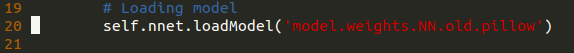
\includegraphics[scale=0.53]{load_model.png}
    \caption*{String to change}
    \label{fig:theModel}
\end{figure}


\paragraph*{Edit the file using sed}\mbox{}\\
Also, you can use the sed command to change the file. Navigate to the DRL project directory, then to src folder and run this command to do it:
\begin{tcolorbox}[width=\linewidth]
\verb!drl_model=./models/model.weights.NN.old.pillow # change this value!
\verb!sed -ri "s:(\s*self\.nnet\.loadModel\(').*('\)):\1$drl_model\2:" play.py!
\end{tcolorbox}

\begin{tcolorbox}[colbacktitle=red!40!white, coltitle=black, width=\linewidth, fonttitle=\bfseries, title=WARNING]
Don't change the sed command except for the path to your model, unless you know what you are doing.
\end{tcolorbox}

\subsubsection*{Additional fitting}
In the first version of the DRL project you can't change training configuration easily using config files. But, if you really want to set up your own training parameters, you can do it by editing source files. Below you can see explanation of the most important training parameters and then, instruction how to change them.

\subparagraph*{Training parameters:}
\begin{itemize}
\item \textit{Memory size} - how many samples should we store in memory to take mini-batch from at one step;
\item \textit{Mini-batch size} - how many samples should we take from memory to perform the next learning step;
\item \textit{Decrease of epsilon step} - decreasing rate of epsilon which is responsible for decision to take a random step or a step, predicted by NN;
\item \textit{Number of allowed actions} - number of actions which NN can perform;
\item \textit{Skip frames} - there is too many frames which the emulator produces. Some of them should be skipped;
\item \textit{Maximum sequence length} - maximum number of steps that NN can perform for one game;
\item \textit{Maximum number of episodes} - maximum number of games during training;
\item \textit{Saving counter threshold} - when should the program save the game. Counts relatively to steps performed by NN;
\item \textit{Base model name} - the first part of the name of model which will be generated;
\end{itemize}

\subparagraph*{How to change parameters:}\mbox{}\\
All this parameters are changing in file \textit{DRL/src/main.py}, so navigate to the \textit{src} directory:
\begin{minted}{bash}
cd DRL/src
\end{minted}

In examples below will be used default values for you to be able to restore the initial state. Just change the value of the variable in the first command to change the certain training parameter.
\begin{tcolorbox}[colbacktitle=red!40!white, coltitle=black, width=\linewidth, fonttitle=\bfseries, title=WARNING]
It is supposed that you are working with the unedited version of \textit{"main.py"} of the first version of DRL. If you are not sure, please, don't use this commands. They may take no effect or even corrupt the code. Also, you may change this parameters in your favorite text editor, but it's not recommended. 
\mbox{}\\
\end{tcolorbox}
\mbox{}\\
\textit{Memory size:}
\begin{tcolorbox}[width=\linewidth]
\verb!drl_mem_size=100000 # change this value! \\
\verb!drl_regex='(\s*self\.size\s?=\s?)[0-9]+(\s*#\s?(M|m)emory\ssize)'! \\
\verb!sed -ri "s:$drl_regex:\1$drl_mem_size\2:" main_exp.py!
\end{tcolorbox}

\textit{Minibatch size:}
\begin{tcolorbox}[width=\linewidth]
\verb!drl_minibatch=128 # change this value! \\
\verb!drl_regex='(\s+self\.minibatch_size\s?=\s?)[0-9]+(\s*#\s?(M|m)inibatch\ssize)'! \\
\verb!sed -ri "s:$drl_regex:\1$drl_minibatch\2:" main_exp.py!
\end{tcolorbox}

\textit{Decrease of epsilon step:}
\begin{tcolorbox}[width=\linewidth]
\verb!drl_eps_step=700000 # change this value! \\
\verb!drl_regex='(\s*self\.epsilon_step_dec\s*=\s*)[0-9]+(.*)'! \\
\verb!sed -ri "s|$drl_regex|\1$drl_eps_step\2|" main_exp.py!
\end{tcolorbox}

\textit{Number of allowed actions:}
\begin{tcolorbox}[width=\linewidth]
\verb!drl_actions=4 # change this value! \\
\verb!drl_regex='(\s+self\.number_of_actions\s?=\s?)[0-9]+(\s*#\s?(L|l)eft,?\sright.*)'! \\
\verb!sed -ri "s:$drl_regex:\1$drl_actions\2:" main_exp.py!
\end{tcolorbox}

\textit{Skip frames:}
\begin{tcolorbox}[width=\linewidth]
\verb!drl_skipframes=6 # change this value! \\
\verb!drl_regex='(\s*self\.ale\s*=\s*ALE\(self\.memory,\sskip_frames=)[0-9]+(\).*)'! \\
\verb!sed -ri "s|$drl_regex|\1$drl_skipframes\2|" main_exp.py!
\end{tcolorbox}

\textit{Maximum sequence length:}
\begin{tcolorbox}[width=\linewidth]
\verb!drl_max_seqlength=50000 # change this value! \\
\verb!drl_regex='(\s+while\sself\.T\s<\s)[0-9]+(\sand\snot\sself\.ale\.game_over:)'! \\
\verb!sed -ri "s|$drl_regex|\1$drl_max_seqlength\2|" main_exp.py!
\end{tcolorbox}

\textit{Maximum number of episodes:}
\begin{tcolorbox}[width=\linewidth]
\verb!drl_max_episodes=50000000 # change this value! \\
\verb!drl_regex='(\s+while\sself\.M\s<\s)[0-9]+(:)'! \\
\verb!sed -ri "s|$drl_regex|\1$drl_max_episodes\2|" main_exp.py!
\end{tcolorbox}

\textit{Saving counter threshold:}
\begin{tcolorbox}[width=\linewidth]
\verb!drl_count_threshold=20000 # change this value! \\
\verb!drl_regex='(\s+if\sself\.count\s>=\s)[0-9]+(:)'! \\
\verb!sed -ri "s|$drl_regex|\1$drl_count_threshold\2|" main_exp.py!
\end{tcolorbox}

\textit{Base model name:}
\begin{tcolorbox}[width=\linewidth]
\verb!drl_model_name=AS.model.weights.NN.NMem # change this value! \\
\verb!drl_regex='(self\.nnet\.saveModel\('\.\/models\/).*(\.'\s\+\sstr\(self\.steps\)\)'! \\
\verb!sed -ri "s|$drl_regex|\1$drl_model_name\2|" main_exp.py!
\end{tcolorbox}

To revert all changes:
\begin{tcolorbox}[width=\linewidth]
\verb!drl_regex='(\s*self\.size\s?=\s?)[0-9]+(\s*#\s?(M|m)emory\ssize)'! \\
\verb!sed -ri "s:$drl_regex:\1100000\2:" main_exp.py! \\
\verb!drl_regex='(\s+self\.minibatch_size\s?=\s?)[0-9]+(\s*#\s?(M|m)inibatch\ssize)'! \\
\verb!sed -ri "s:$drl_regex:\1128\2:" main_exp.py! \\
\verb!drl_regex='(\s*self\.epsilon_step_dec\s*=\s*)[0-9]+(.*)'! \\
\verb!sed -ri "s|$drl_regex|\1700000\2|" main_exp.py! \\
\verb!drl_regex='(\s+self\.number_of_actions\s?=\s?)[0-9]+(\s*#\s?(L|l)eft,?\sright.*)'! \\
\verb!sed -ri "s:$drl_regex:\14\2:" main_exp.py! \\
\verb!drl_regex='(\s*self\.ale\s*=\s*ALE\(self\.memory,\sskip_frames=)[0-9]+(\).*)'! \\
\verb!sed -ri "s|$drl_regex|\16\2|" main_exp.py! \\
\verb!drl_regex='(\s+while\sself\.M\s<\s)[0-9]+(:)'! \\
\verb!sed -ri "s|$drl_regex|\150000000\2|" main_exp.py! \\
\verb!drl_regex='(\s+while\sself\.T\s<\s)[0-9]+(\sand\snot\sself\.ale\.game_over:)'! \\
\verb!sed -ri "s|$drl_regex|\150000\2|" main_exp.py! \\
\verb!drl_regex='(\s+if\sself\.count\s>=\s)[0-9]+(:)'! \\
\verb!sed -ri "s|$drl_regex|\120000\2|" main_exp.py! \\
\verb!drl_regex="(self\.nnet\.saveModel\(\'\.\/models\/).*(\.\'\s\+\sstr\(self\.steps\)\))"! \\
\verb!sed -ri "s|$drl_regex|\1AS.model.weights.NN.NMem\2|" main_exp.py!
\end{tcolorbox}

\section[Experiments]{Experiments}
The model was trained with 900000 steps on NVIDIA GeForce GTX 880M. The training time was two days. This model was compared to random action model. The trained model, as expected, showed better results. The analysis consists of two comparisons: of total rewards for 1000 steps and of average games rewards for 1000 steps. 

The experiment was evaluated on 100000 steps. For one hit, the agent gets reward equals 1. On graphs, one point - is result for 1000 steps. On the ``Y'' axes there is a reward and on the ``X'' axes there is a number on batch.

Below you can see raw results for the random action model (Figures \ref{fig:random}):

\begin{figure}[H]
\centering
\minipage{1\textwidth}
  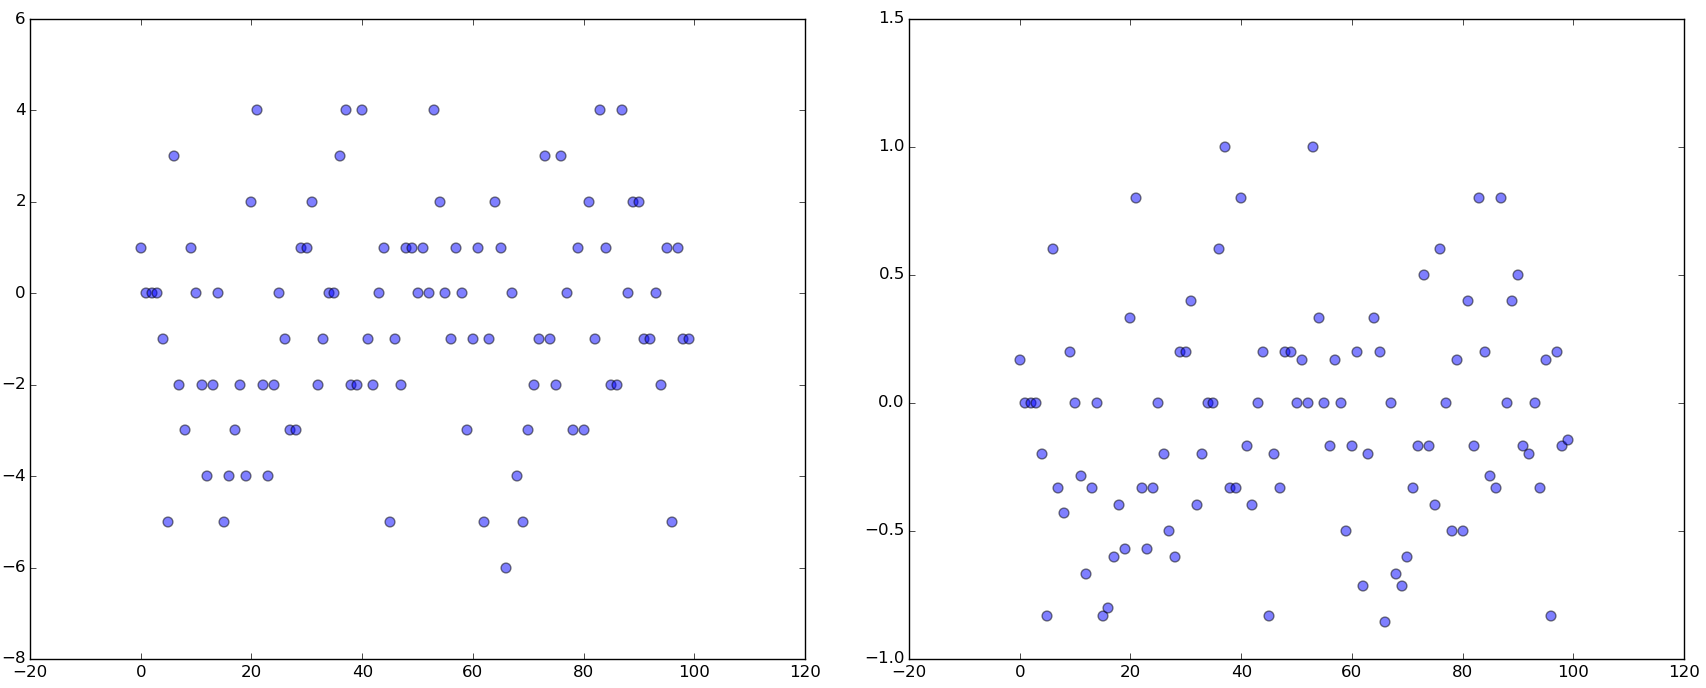
\includegraphics[width=\linewidth]{random.png}
  \caption{Random action model. Left - rewards for 1000 iterations; Right - average rewards for 1 finished game.}\label{fig:random}
\endminipage\hfill
\end{figure} 


The graphs shows expected behavior. Mean rewards are around 0.

But for the trained model - rewards are higher (Figures \ref{fig:trained}):

\begin{figure}[H]
\centering
\minipage{1\textwidth}
  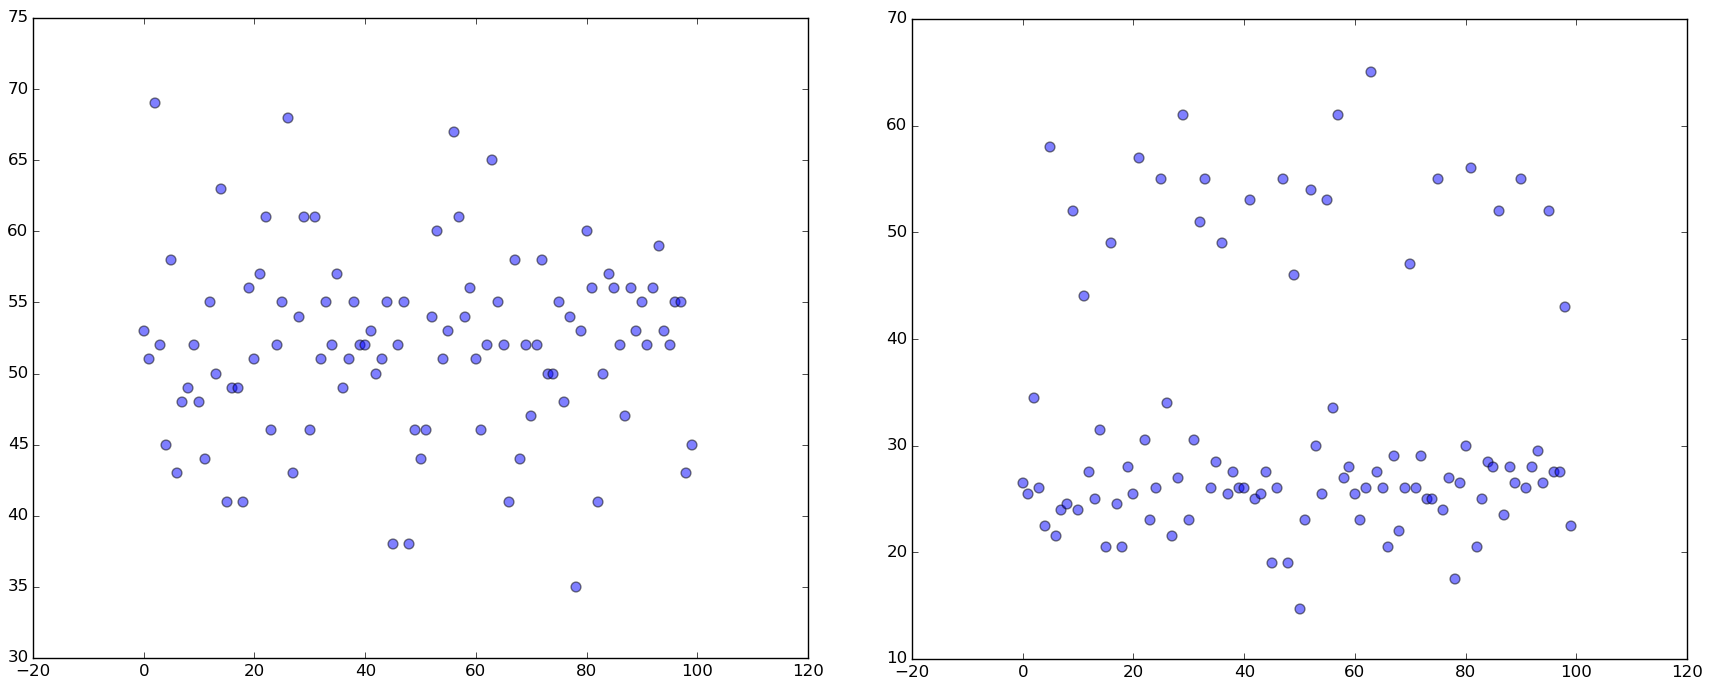
\includegraphics[width=\linewidth]{trained.png}
  \caption{Trained model. Left - rewards for 1000 iterations; Right - average rewards for 1 finished game.}\label{fig:trained}
\endminipage\hfill
\end{figure} 

This graphs shows different behavior. Mean rewards are around 32 which is higher than the random action model results.

In the the Table \ref{table:comparing} below statistical information about the models is presented:

\begin{table}[H]
    \centering
    \begin{tabular}{ | l | l | l | l | l | }
    \hline
     & Random rewards & Random averages & Trained rewards & Trained averages \\ \hline
    Min & -6 & -0.85 & 35 & 14.67 \\ \hline
    Max & 4 & 1.0 & 69 & 65.0 \\ \hline
    Mean & -0.62 & -0.08 & 52.0 & 32.32 \\ \hline
    Median & -1.0 & -0.15 & 52.0 & 27.0 \\ \hline
    STD & 2.35 & 0.42 & 6.32 & 12.42 \\ \hline
    Variance & 5.53 & 0.18 & 40.0 & 154.19 \\ \hline
    \end{tabular}
    \caption{Comparing}
    \label{table:comparing}
\end{table}

Figures \ref{fig:compared_rewards} and \ref{fig:compared_averages} below
\footnote{\url{http://en.wikipedia.org/wiki/Violin_plot}} 
shows relation between results for both models on the same scale. The top figure within each plot is for trained model, and the bottom one is for random action model. The median is marked with a bold dotted line on each figure.

This diagrams shows that the results of the trained model are higher then results of the random action model.

\begin{figure}[H]
    \centering
    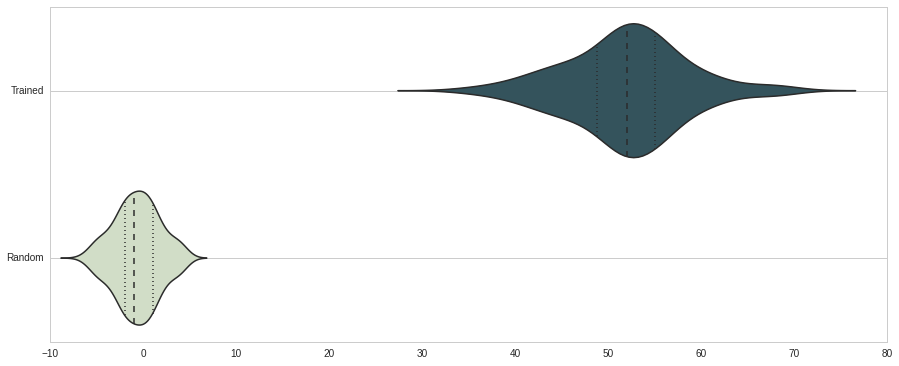
\includegraphics[scale=0.53]{compare_rewards_white.png}
    \caption{Compared rewards}
    \label{fig:compared_rewards}
\end{figure}

\begin{figure}[H]
    \centering
    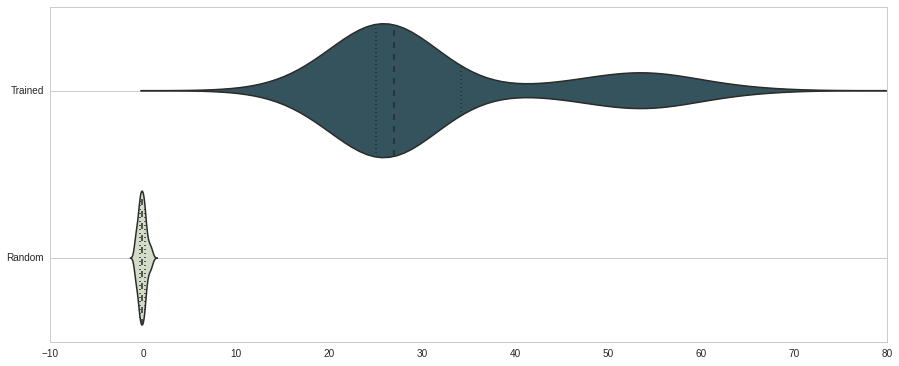
\includegraphics[scale=0.53]{compare_rgstats_white.png}
    \caption{Compared averages}
    \label{fig:compared_averages}
\end{figure}

\end{document}
